\chapter{Human detection}
\label{sec:vision}
In this section, the solution adopted for the vision-based human detection part of the project,
the arguments that led to this approach, the assumptions made,
the tests performed and the obtained results are presented. 

\section{Problem definition}
Once the purpose of the vision system has been well defined,
the operating conditions and the environment must be carefully studied in order to find the most suitable solution.
An embedded vision system portable by a drone, robust and fast enough and with low energy consumption is required for the task. 
The searching for people in the sea entails specific problems that must be treated such as:

\begin{enumerate}[itemsep=1mm,topsep=1mm,leftmargin=.35in]
    \label{list: problem_def}
    \item False positives due to any kind of ocean animals or rocks.
    \item Changes in illumination conditions due to outdoors work.
    \item Forecast behavior: wind, rain.
    \item Moving background and platform.
    \item Highly reflective background.
\end{enumerate}%

Therefore, the selection of the hardware and vision algorithm has to be taken consequently with these points.

\section{Equipment}
According to the ideas above and the available resources,
a logically consistent choice seems to go through the image processing options. 
This is due to the fact that any other kind of visual system
(thermal camera, structured light, time of flight measurements, etc) does not fulfill the requirements or turns out to be too expensive.
Hence, a GoPro HERO 3 camera has been chosen as a robust, light and powerful enough solution \cite{ref:GoPro}.
In order to deal with the instability and disruptions caused by the platform,
the camera has been mounted on a Tarot T-2D Brushless Gimbal Kit, whose technical details
can be found in \cite{Ref:Gimbal}, which is used as a stabilizer.

\subsection{GoPro HERO 3}
The technical parameters of the chosen camera model have influenced the way
the vision algorithm has been approached.
The characteristic small focal length of this camera model, together with the flight altitude of the drone,
leads to a wide field of view, and therefore a big scanned area of ocean per frame. 
The high resolution of the frames allows a precise image processing with a low loss of information in
the acquisition even from high altitude.
Its elevated frame rate for video is, however, constrained by the processing time of the vision algorithm,
which has been developed striving for low memory and time consumption since
it processes the images online and it can be the bottleneck of the system.

\subsection{GoPro gimbal}
The installed gimbal Tarot T-2D Brushless Gimbal Kit offers roll and tilt stabilization and has been
configured to point the camera downwards due to its wide FOV. 
By doing this it is ensured that once the drone is offshore the images will only contain a background of the ocean,
facilitating the image processing and speeding up the preprocessing of the pictures.
Furthermore, as said before, the gimbal provides high stability for precise image acquisition and filters
out disruptions on the flight, which allows an easier and more reliable human detection system.


\section{Vision task}
Given the hardware platform, the image processing algorithm must deal with the remaining
problems in order to reach the goal of the system. 
The initial proposals for people detection, based on movement analysis and human morphological
features extraction where discarded after being subjected to more detailed studies. 
The moving platform and the waves made unfeasible a reliable solution based on movement
tracking assuming that the people to be found were moving.
Furthermore, the possibility of the targets being drowning, partially or almost completely
covered by water prevented any kind of solution from succeeding employing morphological analysis. 
In the view of the arguments above, the final solution was decided to perform human skin
detection based on color under the assumption that at least a part of the targets would be floating. 


\subsection{Human skin identification}
In order to guarantee a robust detection, the RGB-H-CbCr human skin color model presented
in \cite{Ref:SkinColorModel} and \cite{Ref:SkinDetection} has been implemented in the algorithm
and applied for image thresholding as introduced in \cite{Ref:SkinDetection}. 

This color model is based on a set of 140 training patches of skin images used to analyze the properties and
distribution of this color in RGB, HSV and YCbCr spaces.  These training pathches has been exposed
to either normal uniform illumination, daylight illumination (outdoors) or flashlight illumination (under dark conditions). 
As a result of the training, specific constraints in the subspaces have been determined,
so that a general skin color model invariant to illumination and ethnicity was yielded. 
The model is given by the set of bounding rules in the three subspaces in 
equations \ref{eq:rule1}, \ref{eq:rule2}, \ref{eq:rule3} and \ref{eq:rule4}, explained below.

The RGB space constraints are obtained from \cite{Ref:SkinColorModel} and represent the skin
color at uniform daylight illumination \ref{eq:rule1}, and under flashlight or daylight lateral
illumination \ref{eq:rule2}. These two excluding conditions are merged into rule A by means of an OR logical condition.
\begin{equation}
		\begin{cases}
		    (R > 95) AND (G > 40) AND (B > 20),& \text{AND}\\
		    (max(R, G, B) - min(R, G, B) > 15), & \text{AND}\\
		    (abs(R - G) > 15) AND (R > G) AND (R > B)
		\end{cases}
		\label{eq:rule1}
\end{equation}
\begin{equation}
		\begin{cases}
		    (R > 220) AND (G > 210) AND (B > 170),& \text{AND}\\
			(|R - G| <= 15) AND (R > B) AND (G > B)
		\end{cases}
	\label{eq:rule2}
\end{equation}

According to \cite{Ref:SkinDetection}, the discrimination in Cb-Cr domain is defined by the constraints showed in \ref{eq:rule3}.  
These boundaries define a 2D region which contains all the skin color pixels. 
Therefore, these conditions must be all fulfilled at the same time, and are therefore combined by and AND to become the second rule B.

\begin{equation}
		\begin{cases}
			Cr \le 1.5862  Cb + 20         \\
			Cr \le 0.3448  Cb + 76.2069     \\
			Cr \le -4.5652  Cb + 234.5652   \\
			Cr \le -1.15 Cb + 301.75       \\
			Cr \le -2.2857 Cb + 432.85
			\end{cases}
		\label{eq:rule3}
\end{equation}

Finally, as explained on this report below, in the HSV space, the hue values shows the strongest
separation between skin and non-skin regions. 
Since as a previous step in the algorithm the H subspace is thresholded dynamically,
this third set of rules for the color model could be neglected. However, for the sake of completeness they are exposed here.
The constraints in equation \ref{eq:rule4} are combined by an OR, becoming rule C.

\begin{equation}
		\begin{cases}
			H < 25   \\
			H > 230
		\end{cases}
	\label{eq:rule4}
\end{equation}

As a result, the three rules must be accomplished by any pixel in the image to be considered human skin,
and so they conform the filter.
This filter is applied after the input has been binary segmented and  ROI's of the white blobs has been selected,
as it will be detailed in the next section.\\

Each ROI will be subjected to the filter, and if it deems the ROI to contain a human it will be noted, otherwise ignored. 
The filter is applied on every pixel of the image, the response of the pixel is saved in a map. 
If the filter response deems the pixel to be something from a human it will output a white pixel if not a it will output a black pixel.  
If the percentage of white pixels in the ROI is above a threshold value, will it deemed as a human.
An example of successful filtering can be seen in images \ref{fig:humanAndDolphin} and \ref{fig:responsemap}. 

\begin{figure}[H]
    \centering
        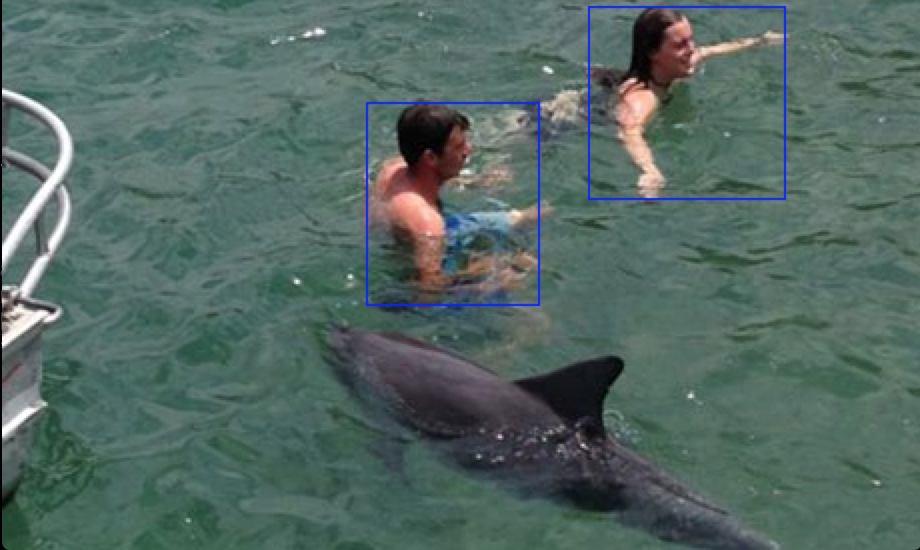
\includegraphics[scale=0.7]{Images/humanDolphin.png}
    \caption{Skin detector capable of distinguishing between animals and humans.}
    \label{fig:humanAndDolphin}
\end{figure}


\begin{figure}[H]
    \centering
    \begin{subfigure}[b]{0.3\textwidth}
    	\centering
			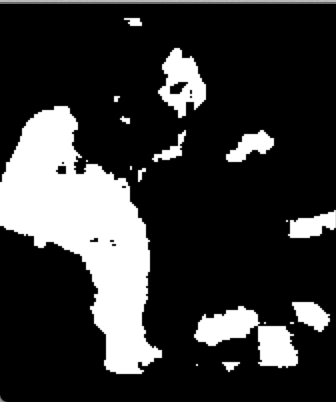
\includegraphics[scale=0.5]{Images/roi_response1.png}
    \end{subfigure}%
    \begin{subfigure}[b]{0.3\textwidth}
    	\centering
			
\includegraphics[scale=0.5]{Images/roi_response2.png}
    \end{subfigure}
    \caption{Response map of the detected ROI, see figure \ref{fig:humanAndDolphin}.}
    \label{fig:responsemap}
\end{figure}

Ordinary detectors such as HaarCascades, are trained to detect people within a certain pose,
as this is a factor which cannot be kept consistent for the application the choice of applying this detector seemed reasonable. \\

Applying these types of filter on a image can be time consuming, esspeacialy if the camera has a wide angled lens.
This issue becomes redundant wihtin this program, as the preproccesing part creates ROI at which the filter can be applied on.
This way is computational time needed shrinken very much,  and make decision of angle of view redundant. \\


\subsection{Preprocessing}
The pixel-wise searching method is a very accurate but heavy process that entails a high time consumption.
In order to speed up the overall performance, some regions of interest in the image with higher possibilities
of containing people must be found as a previous step. 
To do so, an analysis and comparison of example images of the ocean, with and without people and under
different illumination conditions was carried out to determine a procedure to find these regions.

A first approach to this consisted in filtering in the frequency domain in order to remove constant low frequencies,
which would be, in this case, related to the background. Thus, only the high frequency objects would be left, containing all the isolated candidates for the detector.
Notwithstanding, it turned out that a simpler and faster threshold in the hue color space could be set up
to distinguish between floating objects and the background water in all the images. 
These floating objects always involved a disruption or change in the average hue level of the whole picture,
that otherwise remained constant (except for strong glare cases, which will be treated below).
However, a threshold value in hue could not be fixed, due to its dependency with the general illumination level. 
Thus, the solution adopted was to set up a dynamic threshold applying Otsu's method, as described in \cite{Ref:Otsu}.
Proceeding this way, a few small regions containing all the candidates could be input to the skin scan process,
getting rid of the majority of the image with no relevant information. 
This part of the process contains the strongest assumption made for the algorithm. 
For the binarization of the image a uniform background is assumed, meaning that this step will tend to fail for
images with strongly non-homogeneous surroundings. 
It can handle ocean and sky or distant coast lines though. 

Furthermore, an estimation was made here concerning the size of the input ROIs. 
According to flight altitude and the focal length of the camera, an approximate calculation
of the size of the pixel are of people in the image can be made. 
With it all the objects out of this boundaries can be filtered out, easing the posterior process.

As the last point on the preprocessing part, a simple and easy to implement method for dealing with the glare
of the sun light on the water is suggested here, although not implemented in the project, since we came out with this problem at the very end.
The thresholding in hue was proved to fail in the cases of light reflection on small spots for certain intensities,
since this glare effect caused also a strong enough change in the hue image histogram. 
To eliminate these false positives, the easiest solution would be to include a polarizer filter in the setup,
which could also facilitate the color detection. 

\subsection{Postprocessing}
The outputs of the whole process are the images considered to contain people on the water in the patrolled area. 
These pictures are stored and sent to the ground control to be analyzed by the staff in charge,
introducing a human in the control loop.
If the pictures are confirmed to contain people, this means that they are swimming in a forbidden zone or drowning,
and the specific intervention activities are triggered, while the drone keeps its patrol. 

\section{Performance tests}
The design and implementation of the vision algorithm, developed in C++ and OpenCV, has been an iterative
process consisting of several steps of coding and testing of the different parts of the program. 
For testing purposes, a database with several relevant images and videos that fulfilled the specifications for
the application has been created. 
It must be said here that, due to the special characteristics of the problem (listed in \ref{list: problem_def})
and the constraints applied during the design of the vision algorithm to optimize it,
the videos recorded manually trying to emulate similar conditions of the problem failed to help test the program. 
In order to simulate the ocean, a consistent background had to be present in the videos,
but could not be defined for the trials. 

%(some how citation to all images on git and dropbox as it being the database of image)

The following example of successful test for an image in the PC deploys in Figures \ref{fig:original_final},
\ref{fig:HSV}, \ref{fig:threshold} and \ref{fig:ROIs} the main outputs of the intermediate processes explained above,
together with the initial image and the final result. 

\begin{figure}[h]
        \centering
        \begin{subfigure}[h]{0.3\textwidth}
                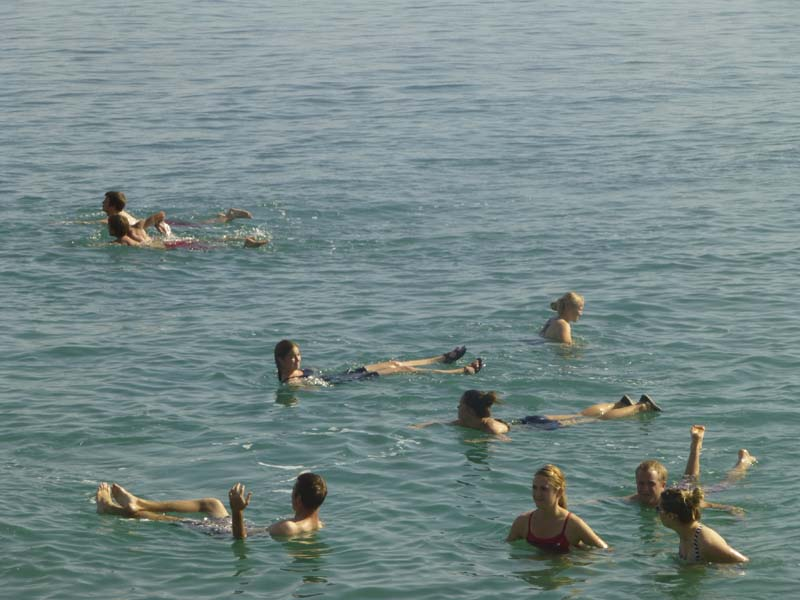
\includegraphics[width=\textwidth]{Images/ocean7}
                \caption{Image 1: original image}
        \end{subfigure}%
        \quad
        \begin{subfigure}[h]{0.3\textwidth}
                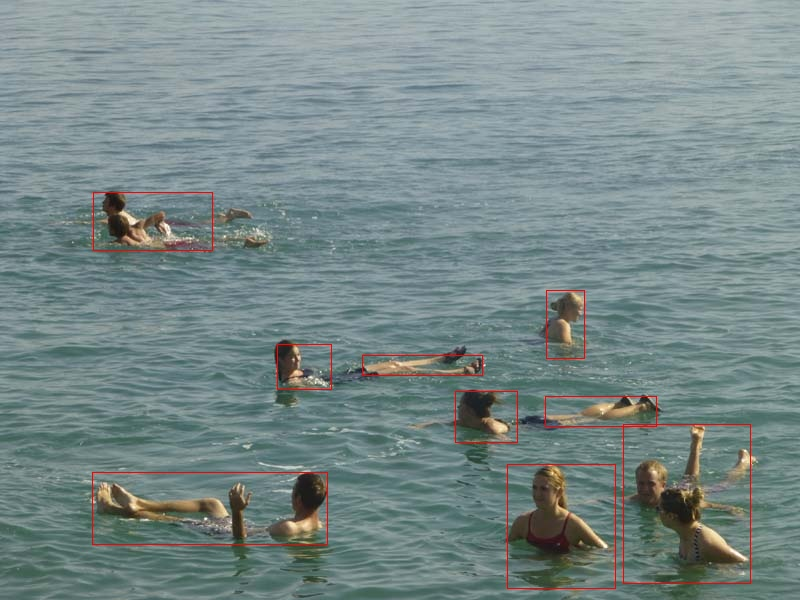
\includegraphics[width=\textwidth]{Images/final}
                \caption{Image 1: processed image}
        \end{subfigure}
        \caption{Original and processed images}
        \label{fig:original_final}
\end{figure}

\begin{figure}[h]
        \centering
        \begin{subfigure}[h]{0.3\textwidth}
                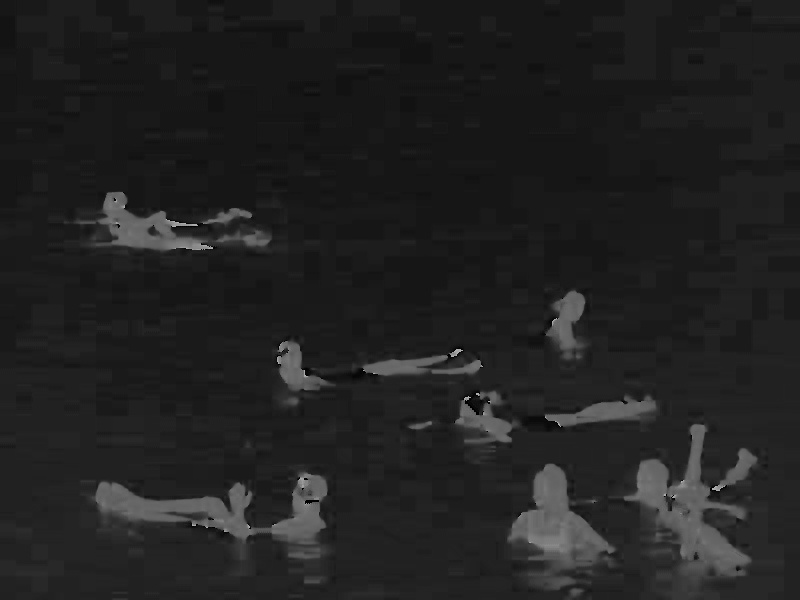
\includegraphics[width=\textwidth]{Images/hue}
                \caption{Image 1: hue}
        \end{subfigure}%
        \quad
        \begin{subfigure}[h]{0.3\textwidth}
                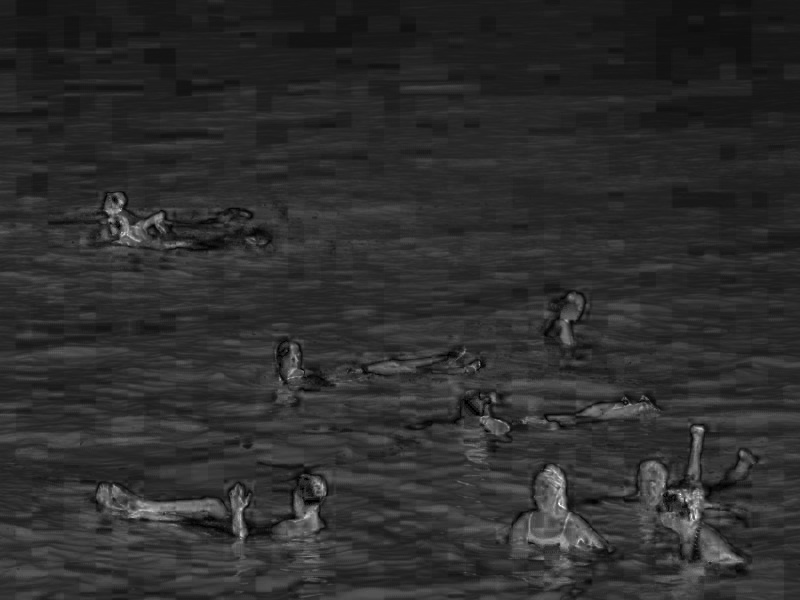
\includegraphics[width=\textwidth]{Images/sat}
                \caption{Image 1: saturation}
        \end{subfigure}
        \quad
        \begin{subfigure}[h]{0.3\textwidth}
                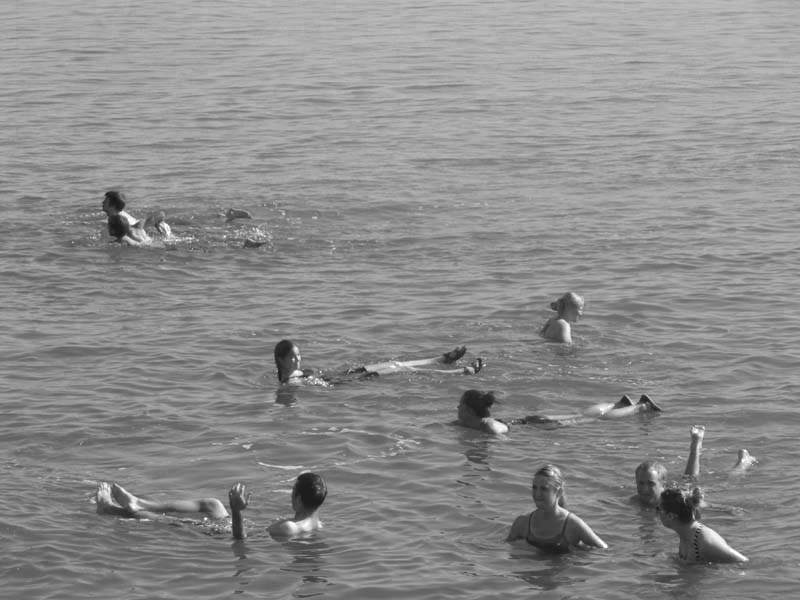
\includegraphics[width=\textwidth]{Images/val}
                \caption{Image 1: value}
        \end{subfigure}
        \caption{HSV color space decomposition}
        \label{fig:HSV}
\end{figure}

\begin{figure}[h]
        \centering
        \begin{subfigure}[h]{0.3\textwidth}
                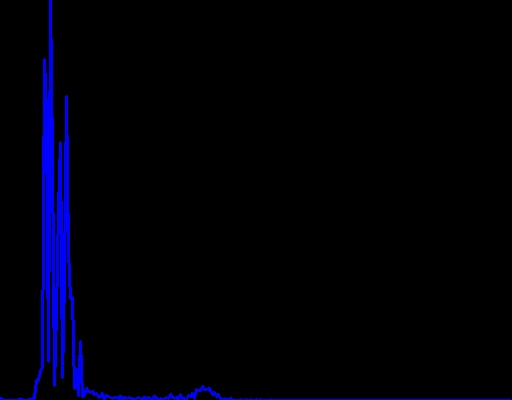
\includegraphics[width=\textwidth]{Images/hueHist}
                \caption{Image 1: hue histogram}
        \end{subfigure}%
        \quad
        \begin{subfigure}[h]{0.3\textwidth}
                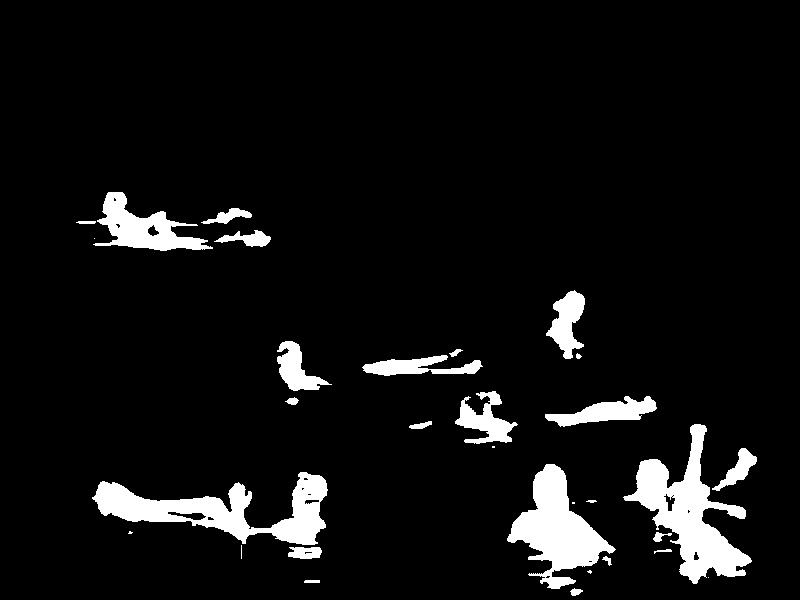
\includegraphics[width=\textwidth]{Images/bin}
                \caption{Image 1: binarized}
        \end{subfigure}
        \caption{Dynamic thresholding in hue}
         \label{fig:threshold}
\end{figure}

\begin{figure}[h]
        \centering
        \begin{subfigure}[h]{0.3\textwidth}
                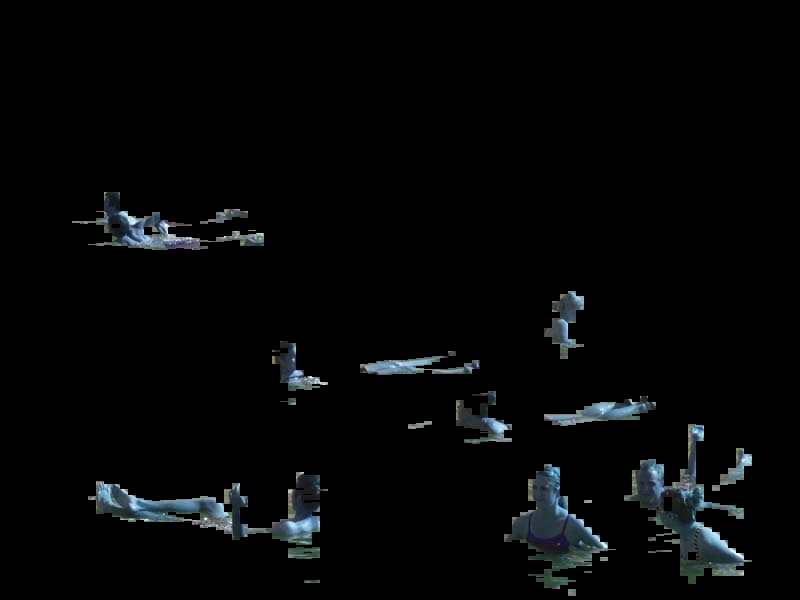
\includegraphics[width=\textwidth]{Images/proc}
                \caption{Image 1: ROIs before particles filtering}
        \end{subfigure}%
        \quad
        \begin{subfigure}[h]{0.3\textwidth}
                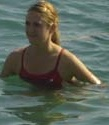
\includegraphics[width=\textwidth]{Images/ROI}
                \caption{Image 1: one of the ROIs amplified after filtering}
        \end{subfigure}
        \caption{Example of region of interest extracted.}
         \label{fig:ROIs}
\end{figure}


\section{Results}
The developed vision system has proved to be robust and reliable for the stated problem.
Its use mounted on a drone, although not tested, can be assumed to be successful since the sum
of the developed and tested parts should result in a working system.
The OpenCV application resulting of the implementation of the algorithm designed demonstrates to be able to filter out animals,
rocks and boats and detect humans off shore under the stated assumptions. 
In addition it can deal automatically with illumination variations, disruption on the platform and glare effects.
However, there are still some particular and very seldom cases in which the vision process fails. 
These mistakes are not critical though since the process includes, as said in the statement of the project,
a human in the control loop, who will be, in the last case, the one in charge of filtering out false detections before activating rescue procedures.

\section{Summary}

An algorithm capable of detection human far away in the ocean has been developed. 
The algorithm uses a skin color model to detect humans,
making it robust and able to distinguish between a human other items.
The skin color model, from the report \cite{Ref:SkinDetection} is based from different form of illuminations, 
making it somewhat invariant to illumination differences. 
The algorithm has been tested with different images found on the internet,
at which it perform well. It is capable of distinguishing between humans and animals as seen in figure \ref{fig:humanAndDolphin}.
The chosen hardware works well on a moving background,
and is thereby capable of retrieving useful footage for analysis. 

\subsection{Further work} 
In order to constrain the scope of the project, it was assumed from the beginning that a successful offline
performance of the application in a laptop processing a video could be extrapolated to good results for online performance. 
According to this, the tests have been carried out making use of acquired or downloaded videos.
As future work, it is left the implementation of the necessary hardware on the drone in order to stream the video
and send it to the ground control to be treated.
It is suggested the use of an added board such as a variant of the Raspberry Pi or similar, together with a USB Wifi adapter.
This setup would provide an easy to install and fast connection for video streaming that would solve the communication.
Furthermore, the ultimate test for the system to be subjected to would be the treatment of a video of the defined scenario acquired by itself. 



\newpage
